%!TEX root = ../document.tex
\chapter{相关理论与技术分析}
% \section{推荐系统}





% \subsection{推荐系统存在的问题}

% \textbf{冷启动问题}%

% \textbf{噪音问题}%

% \textbf{数据长尾问题}%


\section{序列感知模型}
序列感知模型是把数据根据时间日期排序之后,按照数据之间的时间先后顺序,发现时间上近邻的数据之间的隐藏关系或数据的周期性变化规律等与时间有关系的一类数据挖掘模型,数据挖掘领域又常称这类模型为时序模型。因此序列感知模型面对的数据必须包含时间戳或者数据的存储形式能够不丢失数据的诞生先后顺序。时序模型数据分析的目的就是为了挖掘出数据之间的内在时间规律,找到这种时间规律之后利用其归纳、类推、演绎未来的数据变化趋势,从而进行建模样本之外的数据预测。
2018年的ACM RecSys中还专门设立了关于序列感知推荐的课程并发布了一篇关于序列感知推荐的研究综述\upcite{Quadrana:2018:SRS:3209219.3209270}
。



\subsection{序列感知推荐任务及场景}

当待分析的数据具有固有的顺序性质,序列学习方法就会在这些应用领域中有用,比较常见的应用有如自然语言处理、语音识别、时间序列预测、DNA建模,以及作为本文工作的核心内容,序列感知推荐。


\section{序列建模技术分类}

% \subsection{频繁集挖掘}

% \subsection{马尔可夫链}

\subsection{循环神经网络}

因为传统前馈深度神经网络(FNN)无法了解给定输入的上下文环境关系,循环神经网络(RNN)\upcite{RNN1994}被发明的目的就是用来进行对可变长度的序列数据进行建模。循环神经网络与传统的FNN模型之间的主要区别在于组成网络的单元中存在内部隐藏状态,在一个序列建模步骤中的每个内部隐藏状态节点都接收来自上一个节点的输入,因此这可以用一个循环来表示,其结构如图\ref{fig:rnn}所示,隐藏状态层保留了过去序列编码的摘要,每当RNN呈现新的输入时,就会更新该隐藏层的状态。对于一个最简单的标准循环神经网络其通过以下形式来更新隐藏单元的状态$h$:
\begin{equation}
  \label{eq:rnn}
  h_{n} = f \left(Ux_{n} + Wh_{n-1} + b \right)
\end{equation}
其中$h_{n-1}$是第$n-1$层神经网络的向量化表示,$x_{n}$是传递给第$n$层的输入序列编码,$U,W$是该层包含的权重矩阵,$b$是该层向量的偏置。函数$f(\cdot)$为非线性转换函数,也称激活函数,常用的激活函数有Logistic Sigmoid函数$\sigma(\cdot )$,$tanh(\cdot)$,线性整流单元$ReLU(\cdot)$和一些它们的变体。经过以上隐藏层状态的更新之后,输出层的计算公式如下:
\begin{equation}
  \label{eq:rnn1}
  \hat{y}_{n} = g(Vh_{n})
\end{equation}
其中$\hat{y}_{n}$是$n$时刻的输出值,$V$是输出层的权重矩阵,$g(\cdot)$是输出层的激活函数。

\begin{figure}[htb]%更改
  \centering
  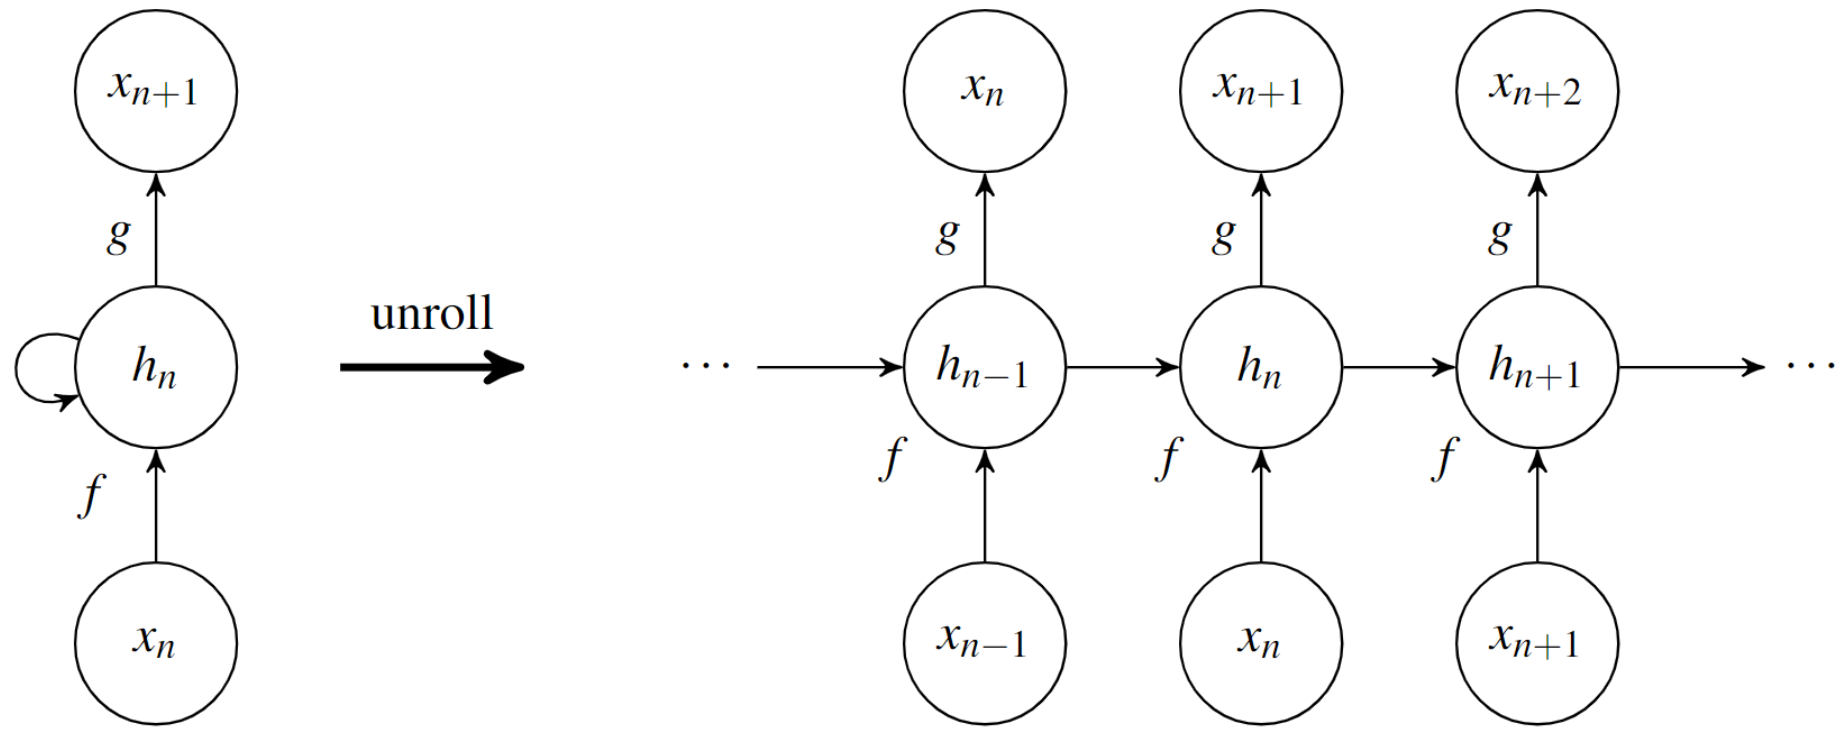
\includegraphics[width=12cm]{rnn.png}\\
  \caption{简单循环神经网络结构图}
  \label{fig:rnn}
\end{figure}

通过公式\ref{eq:rnn},\ref{eq:rnn1}可以明白,RNN的每一个时间步骤都会有一个新的输入,并且特定时间步骤的输出依赖于之前所有步骤的输入,这意味着时间步骤$N$时刻的损失函数的计算要回溯到时间步骤$1$,这一过程也称为\textit{基于时间的反向传播算法(backpropagation through time, BPTT)}\upcite{Sutskever:2013:TRN:2604780}。但是如果要处理的序列很长的话,经过多层的反向传播,BPTT会产生梯度消息或者梯度爆炸的问题,以至于无法从差的很远的时间步骤中感知上下文环境,使得RNN的训练变得非常麻烦,RNN这一明显的缺点也称为长期依赖问题。

\subsection{长短期记忆神经网络}

为了解决RNN的长期依赖问题,一些基于公式\ref{eq:rnn}的变形工作诞生,其中最广为人知的是长短期记忆网络(long short-term memory, LSTM)\upcite{LSTM1997}。LSTM通过精巧设计的记忆单元更换了RNN中的隐藏单元,其核心计算单元如图\ref{fig:lstm}所示。LSTM神经元内部通过精心设计的分别称为遗忘门、输⼊门、输出门的三个门结构来决定哪些信息更新到内部或者从内部去除。在遗忘门\eqref{forget_gate}当中,前一时间步的掩藏状态和当前时间步的输入经过Sigmoid函数非线性转换之后得到一个$[0,1]$之间的值,以表示需要遗忘信息的概率。在输入门\eqref{input_gate},\eqref{input_gate1}中,将当前时间步骤中的输入和前一时间步骤学习到的隐藏状态经过tanh激活函数的计算生成一些候选值,并通过Sigmoid函数的传递从候选值中选出一些进行更新。而输出门\eqref{output_gate}就决定了当前单元要输出哪些部分。LSTM通过如下的组合函数来更新隐藏单元的状态:
  \begin{align} 
  f_{t} &=\sigma(U_{f} x_{t}+W_{f}[h_{t-1}+ c_{t-1}] +b_{f}) \label{forget_gate}\\
  i_{t} &=\sigma(U_{i} x_{t}+W_{i}[h_{t-1}+ c_{t-1}]+b_{i}) \label{input_gate}\\  
  c_{t} &=f_{t} c_{t-1}+i_{t} \tanh (U_{c} x_{t}+W_{c} h_{t-1}+b_{c}) \label{input_gate1}\\ 
  o_{t} &=\sigma(U_{o} x_{t}+W_{o}[h_{t-1}+ c_{t}]+b_{o}) \label{output_gate}\\ 
  h_{t} &=o_{t} \tanh (c_{t}) 
  \end{align}
% \end{equation}

其中$\sigma(\cdot)$是Logistic Sigmoid激活函数;而$i$、$f$、$o$和$c$分别是输入门、遗忘门、输出门和隐藏层的激活向量;变量$b$表示偏置向量,例如$b_{f}$表示为遗忘门的偏置向量。$U$、$W$分别代表输入向量的权重和上一层输出的权重,例如在遗忘门中,$U_{f}$代表遗忘门输入向量$x_{t}$的权重,$W_{f}$代表上一个LSTM神经元输出$h_{t-1}$的权重。

\begin{figure}[htb]
  \centering
  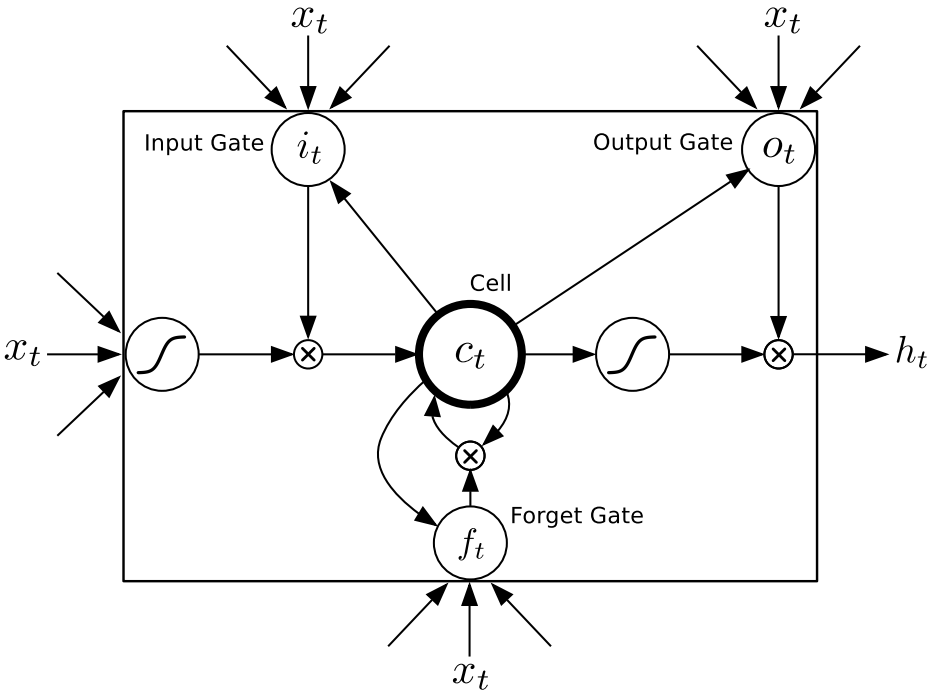
\includegraphics[width=12cm]{lstm.png}\\
  \caption{长短期记忆网络神经元结构图}
  \label{fig:lstm}
\end{figure}

\subsection{门控循环单元}

由于LSTM在循环神经单元中增加了三个门结构,与RNN相比,在一个神经元当中要完成更多的复杂计算。当使用更大的网络的时候,训练时间相比RNN也将显著增加。为了减少训练的时间复杂度并同时保留LSTM对长期依赖关系的记忆能力,2014年Cho等人提出门控循环单元(Gated Recurrent Unit, GRU)\upcite{GRU2014}。与LSTM相似,GRU使用门结构建模单元内部信息的流动,不同的是,GRU将LSTM三个门减少为两个。GRU使用更新门来决定是否遗忘上时刻的信息或者记忆此时刻新的外部输入信息,其功能相当于组合了LSTM 中的输入门与遗忘门。使用重置门来决定如何将新的输入信息与内部已有放入记忆相结合。在$t$时刻GRU单元中更新门的状态表达式为:
$$
z_{t}^{j}=\sigma\left(U_{z} \mathbf{x}_{t}+W_{z} \mathbf{h}_{t-1}\right)^{j}
$$
其中,$\mathbf{x}_{t}$为第$t$个时间步骤的输入向量,$\mathbf{h}_{t-1}$中保存的是上一个时间步骤的信息。$U$,$W$是更新门当中输入向量与上一时间步信息的权重矩阵。$t$时刻GRU单元中重置门为:
$$
r_{t}^{j}=\sigma\left(U_{r} \mathbf{x}_{t}+W_{r} \mathbf{h}_{t-1}\right)^{j}
$$
结合更新门与重置门,整个GRU神经元在$t$时间步的内部状态更新为:
$$
z_{t}^{j}=\sigma\left(U_{z} \mathbf{x}_{t}+U_{z} \mathbf{h}_{t-1}\right)^{j}
$$
其中$\tilde{h}_{t}^{j}$为候选信息,表示当前记忆的内容,其计算表达式为:
$$
h_{t}^{j}=\left(1-z_{t}^{j}\right) h_{t-1}^{j}+z_{t}^{j} \tilde{h}_{t}^{j}
$$
单个GRU神经元的总体结构如图\ref{fig:gru}所示。

\begin{figure}[htb]
  \centering
  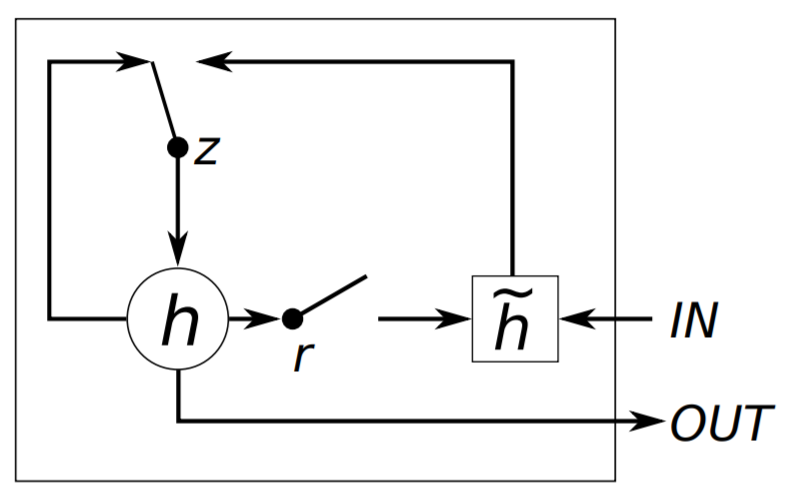
\includegraphics[width=12cm]{gru.png}\\
  \caption{门控循环单元神经元结构图}
  \label{fig:gru}
\end{figure}

\subsection{双向循环神经网络}

在自然语言处理的实体识别技术中,双向循环神经网络(Bidirectional recurrent neural networks, BRNN)\upcite{Schuster1997BidirectionalRN}弥补了单项循环神经网络对于上下文感知能力的不足,因为单向RNN预测下一个单词时使用的只是此单次出现之前的信息,而BRNN则从两个方向获取信息,上下文感知能力也就更强了。BRNN将隐藏层分为两个部分,前向状态层$\stackrel{\rightarrow}{h}$和反向状态层$\stackrel{\leftarrow}{h}$,其输出层的输入由$\stackrel{\rightarrow}{h}$和$\stackrel{\leftarrow}{h}$堆叠而成,其迭代公式如下:
\begin{align} 
  \vec{h}_{t} &= \sigma(U_{\vec{h}} x_{t}+W_{\vec{h} \vec{h}} \vec{h}_{t-1}+b_{\vec{h}}) \label{forword}\\
\stackrel{\leftarrow}{h}_{t} &= \sigma(U_{\stackrel{\leftarrow}{h}} x_{t}+W_{\stackrel{\leftarrow}{h} \stackrel{\leftarrow}{h}} \stackrel{\leftarrow}{h}_{t+1}+b_{\stackrel{\leftarrow}{h}}) \label{backword}\\
y_{t} &= W_{\vec{h} y} \vec{h}_{t}+W_{\stackrel{\leftarrow}{h}y} \stackrel{\leftarrow}{h}_{t}+b_{y} \label{stack}
\end{align}

BRNN的隐藏层结构如图\ref{fig:brnn}所示。
\begin{figure}[htb]
  \centering
  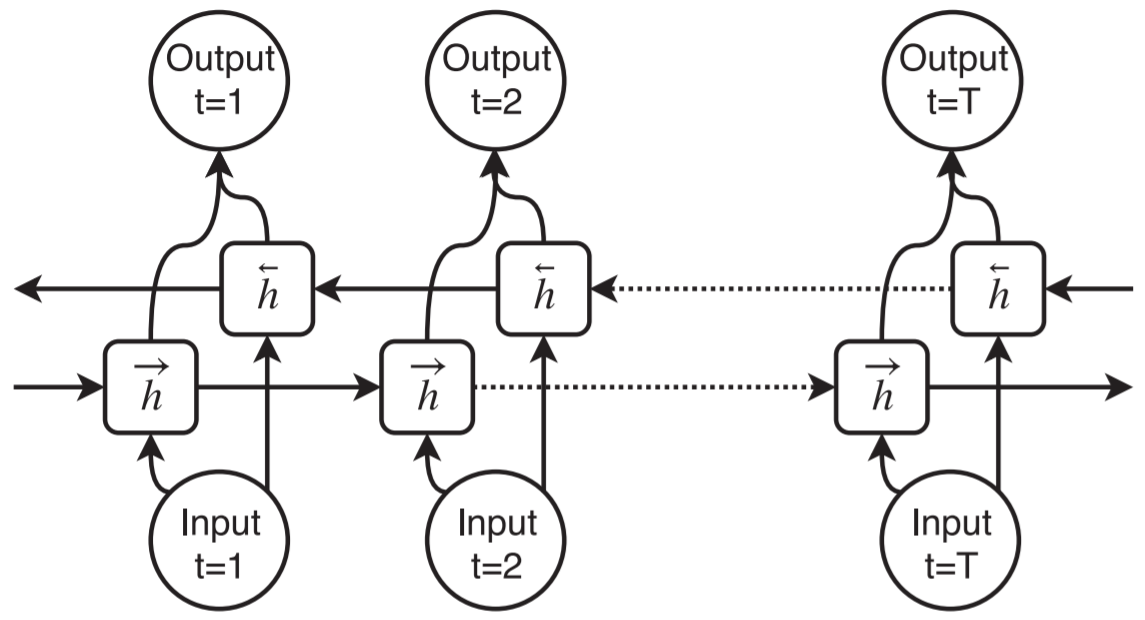
\includegraphics[width=12cm]{brnn.png}\\
  \caption{双向循环网络神经结构图}
  \label{fig:brnn}
\end{figure}

\subsection{时间卷积网络}
卷积神经网络通常用于计算机视觉领域的图像特征提取,将其应用于序列建模需要对卷积神经网络的结构做出修改,目前将卷积神经网络运用于序列建模的最良好算法为2018年Shaojie Bai等人提出的时间卷积网络(Temporal Convolutional Network,TCN)\upcite{TCN2018},本文在此把TCN作为CNN在序列建模领域的代表。

TCN由因果卷积(Causal Convolution)、扩张卷积(Dilated Convolution)和残差链接(Residual Connection)三部分构成。

\textbf{因果卷积}
在序列建模任务中,首先得保证输入序列与输出序列的长度一直,因此在TCN中使用的卷积结构是1维全卷机网络,其中每一个隐藏层的长度都与输入层长度相同,对于经过卷积过滤器计算的中间隐藏层,长度会减小,通过0填充的方式使其扩充到长度相等。如果直接对输入序列进行卷积操作的话,卷积操作将会是对序列的全局进行计算,这会导致信息泄露的问题,即在训练时让现在时刻知道了未来时刻的信息,而这种情况面对真实世界时是不可能发生的。为了防止训练时将未来时刻信息泄露到了现在时刻,因果卷积被引入。所谓因果卷积, 就是计算$t$时刻的输出时, 仅对前一层$t$时刻及之前的状态进行卷积。因果卷积等价于掩码卷积(masked convolution)\upcite{DBLP:journals/corr/OordKK16},在输入序列上加上掩码把未来时刻的信息对现在时刻进行屏蔽。

\textbf{扩张卷积}
对于因果卷积,如果需要获得更大的感受野来捕获更长范围的序列的话需要很多层或者很大的过滤器,为了更加因果卷积的感受野,扩张卷积被引入与其结合。扩张卷积通过跳过部分输入来使过滤器能应用于比过滤器本身大小更大的范围,等同于通过0填充来扩大原先的过滤器。
Dilation convolution的运算如下:
$$
  F(s)=\left(\mathbf{x} *_{d} f\right)(s)=\sum_{i=0}^{k-1} f(i) \cdot \mathbf{x}_{s-d \cdot i}
$$
其中$\mathbf {x}$表示输入序列, $f$ 表示 过滤器filter, $d$ 是扩张因子,%
 $k$ 是过滤器大小,  $s-d\cdot i$意味着只对过去的状态作卷积。图\ref{fig:TCN}为结合了因果操作和扩张操作的卷积示意图。
\begin{figure}[htb]
  \centering
  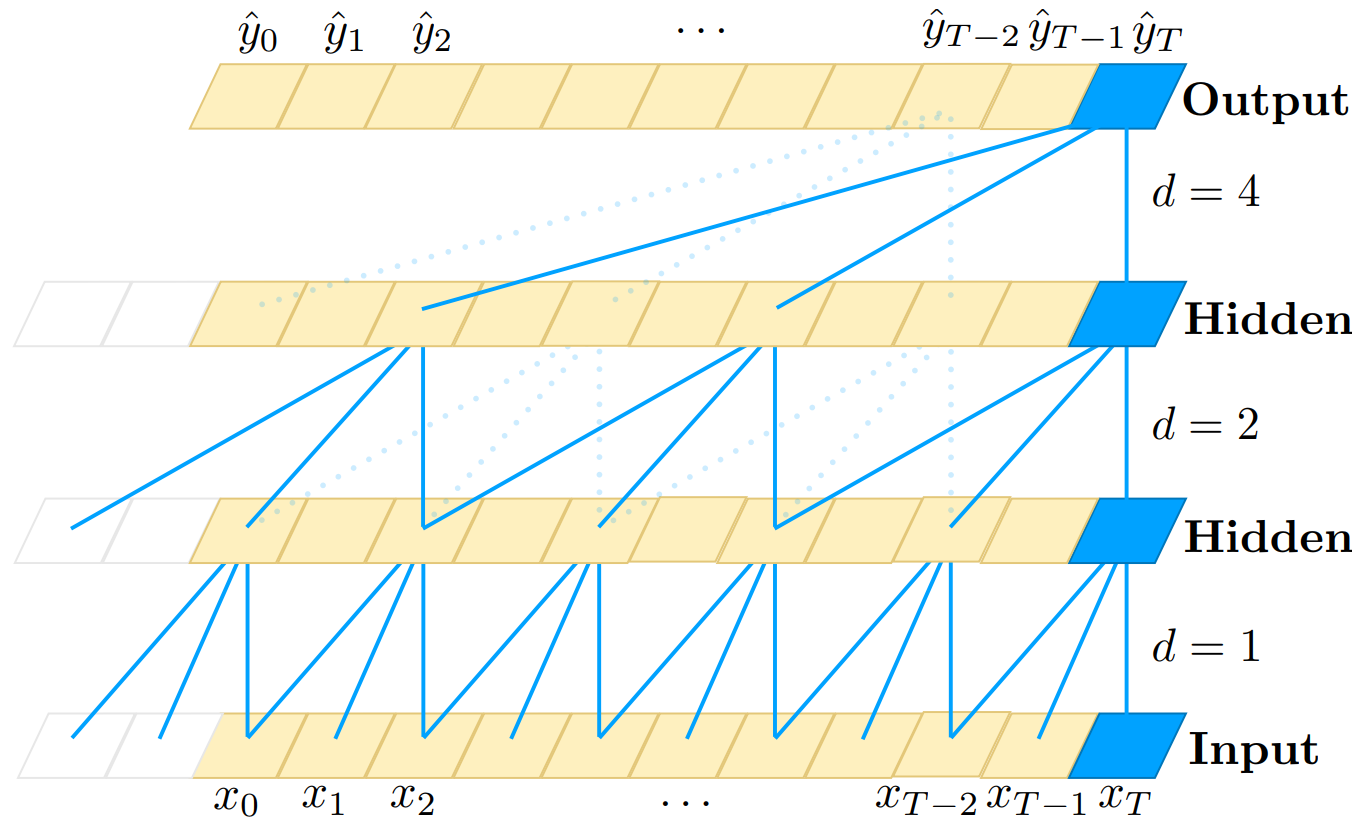
\includegraphics[width=\linewidth]{TCN.png}\\
  \caption{扩张因子分别为1,2,4和过滤器大小为3的扩张因果卷积网络结构图}
  \label{fig:TCN}
\end{figure}

\textbf{残差链接}
由于卷积神经网络对序列建模能记忆的时间步长度依赖于网络的深度,TCN为了获得更大的感受野,因此不得不增加网络的深度。为了使深层网络的训练不至于丢失浅层特征,残差连接是用来解决这个问题的常用办法,因此TCN结构中加入了残差连接以增加网络深度。
\begin{align}
  o=\operatorname{Activation}(\mathbf{x}+\mathcal{F}(\mathbf{x}))
\end{align}
其中$\mathcal{F}(\cdot)$为残差结构略过的深层隐藏网络。残差网络通过建立输入与输出之间的捷径网络,使有效的浅层特征能够直接传递给输出层,避免了所有特征向量都必须经过深层隐藏网络的计算,保留了浅层有效特征,使得训练深层网络变得更加容易。


% \subsection{序列感知推荐算法评价指标}

\subsection{注意力机制}
在自言语言处理的机器翻译算法中,有一类端到端的模型有着出色的性能。
而为了说明深度学习中的注意力模型,就不得不先谈这一类端到端框架,因为目前大多数注意力模型都作为端到端框架下的一部分使用。
其中代表工作为2014年Ilya Sutskever等人提出的Seq2Seq\upcite{DBLP:journals/corr/GehringAGYD17}模型,Seq2Seq有一个编码器(Encoder)和一个解码器(Decoder)构成。
% \section{序列感知推荐}

Seq2Seq模型中把序列建模问题当做一个条件概率问题:
\begin{align}
  p\left(y_{i} | y_{1}, \ldots, y_{i-1}, \mathbf{x}\right)=g\left(y_{i-1}, s_{i}, c_{i}\right)
\end{align}
其中$s_{i}$为Decoder中$i$时刻的状态,其计算公式为:$s_{i}=f\left(s_{i-1}, y_{i-1}, c_{i}\right)$,
$c_{i}$为该时刻状态的权重,其计算公式为$c_{i}=\sum_{j=1}^{T_{x}} \alpha_{ij} h_{j}$,其中$i$表示Encoder端的第$i$时刻输入。
$h_{j}$表示Encoder端的第$j$个输入的隐向量,$\alpha_{i j}$表示Encoder端的%
第$j$个输入与Decoder端的第$i$个输入之间的权值,表示源端第$j$个输入对目标端%
第$i$个输入的影响程度,$\alpha_{i j}$的计算公式如公式\eqref{attention}所示:
\begin{align}
  \alpha_{i j}=\frac{\exp \left(e_{i j}\right)}{\sum_{k=1}^{T_{x}} \exp \left(e_{i k}\right)} \label{attention}
\end{align} 
其中$e_{i j}=a\left(s_{i-1}, h_{j}\right)$。

在公式\eqref{attention}中,$\alpha_{ij}$是一个softmax模型输出,概率值的和为1。%
$e_{ij}$表示一个对齐模型,用于衡量Encoder端的位置$j$个词,对于Decoder端的位置%
$i$个词的对齐程度(影响程度),换句话说:Decoder端生成位置i的词时,有多少程度受%
Encoder端的位置$j$的词影响。对齐模型$e_{ij}$的计算方式有很多种,不同的计算方式,代表不同%
的Attention模型,最简单且最常用的的对齐模型是dot product乘积矩阵,即把target端%
的输出隐状态ht与source端的输出隐状态进行矩阵乘。常见的对齐计算方式如下:
\begin{align}
\operatorname{score}\left(\boldsymbol{h}_{t}, \overline{\boldsymbol{h}}_{s}\right)=
\left\{
  \begin{array}{ll}{\boldsymbol{h}_{t}^{\top} \overline{\boldsymbol{h}}_{s}} & {\text { dot }} \\ {\boldsymbol{h}_{t}^{\top} \boldsymbol{W}_{a} \overline{\boldsymbol{h}}_{s}} & {\text { general }} \\ {\boldsymbol{v}_{a}^{\top} \tanh \left(\boldsymbol{W}_{\boldsymbol{a}}\left[\boldsymbol{h}_{t} ; \overline{\boldsymbol{h}}_{s}\right]\right)} & {\text {concat}}
  \end{array}
\right.
\end{align} 

\section{本章小结}

本章主要围绕序列感知推荐算法中关键的序列建模技术进行论述,先简要介绍了序列建模技术广泛的应用%
领域,对序列建模理论引入推荐算法领域的可能性进行了铺垫,然后对后文中涉及到的关键技术和理论进行%
简要概述,从RNN、CNN、Attention三个大的层次上对当前领域内使用比较多的序列建模基础技术RNN、LSTM、GRU、BRNN、TCN、Attention Mechanism等原理进行了详细介绍,通过完整的理论支撑充分证明了本文的可行性。
